
\section{Math library}
\label{section_math_library}
\subsection{Math expressions in coordinates and domains}
"pgfplots" loads a math library that is part of the Tikz bundle. Among
other things it allows you to make calculations within coordinates and
domains:
\begin{latex}
\begin{tikzpicture}
\begin{axis}[xmin=0,xmax=11,ymin=0,ymax=6]
\draw (1,1) -- "(2*5,6-2/2)";
\end{axis}
\end{tikzpicture}
\end{latex}
%
\begin{center}
\tikzcount
\begin{tikzpicture}
\begin{axis}[xmin=0,xmax=11,ymin=0,ymax=6]
\draw (1,1) -- (2*5,6-2/2);
\end{axis}
\end{tikzpicture}
\end{center}
Sometimes you need to enclose the math expression in "{...}" to make
sure it gets parsed (when in doubt, enclose the material in "{...}",
but the manual says it's necessary when the expression contains
"(...)"\ ).
\begin{latex}
\begin{tikzpicture}
\begin{axis}[axis lines = middle,
xmin=-pi/2,xmax=pi,ymin=sin(-90),ymax=sin(90),
trig format plots = rad,"enlargelimits"]
\addplot[very thick,smooth,blue,domain="-pi/2:pi/2"]{sin(x)};
\addplot[mark=*] ("pi/3,{sqrt(3)/2}") % note this is parametric coordinate format
        node[below right]{$(\pi/3,\sqrt{3}/2)$};
\end{axis}
\end{tikzpicture}
\end{latex}
%
\begin{center}
\tikzcount
\begin{tikzpicture}
\begin{axis}[axis lines =
  middle,xmin=-pi/2,xmax=pi,ymin=sin(-90),ymax=sin(90), enlargelimits]
\addplot[very thick,smooth,blue,domain=-pi/2:pi/2]{sin(deg(x))};
\addplot[mark=*] (pi/3,{sqrt(3)/2}) 
        node[below right]{$(\pi/3,\sqrt{3}/2)$};
\end{axis}
\end{tikzpicture}
\end{center}

From the "pgfplots" manual: the operations and functions include
``"+","-" , "*", "/", "abs", "round", "floor", "mod", "<", ">", "max",
"min", "sin", "cos", "tan", "deg" (conversion from radians to
degrees), "rad" (conversion from degrees to radians), "atan", "asin",
"acos", "cot", "sec", "cosec", "exp", "ln", "sqrt", the constants\
"pi" and "e", "^" (power operation), "factorial", "rand" (random
between $-1$ and $1$), "rnd" (random between $0$ and $1$).'' In fact,
there are a fair number more functions, see the 
\href{https://ctan.org/pkg/pgf}{Tikz/PGF manual}.

\subsection{Declaring functions}
As part of the math package Tikz provides (and which is inherited by
"pgfplots"), you can define functions (in the mathematical sense) and
use them in plots.  You can also define constants, which are
essentially functions without any inputs.  The crucial command is %
"declare function", and the crucial syntax to watch out for is that
\emph{each function or constant you define needs to end with }``;''.
You can put %
"declare function" in either the optional arguments to "tikzpicture"
or to "axis".  I tend to put it in "tikzpicture" just because in my
mental space, it comes as early as possible in the overall picture
(I'd put it in the ``preamble'' of the picture if this existed), and
isn't really part of what I'm drawing.

\subsubsection{Quadratic and tangent line}
This is a good way to graph functions and tangent lines, because you
can easily change the point of tangency:
\begin{latex}
\begin{tikzpicture}["declare function = {
a = 2;" % ** everything ** is calculated in terms of this
"f(\x) = \x^2;
fp(\x) = 2*\x;
m = fp(a);}"]
% OK, now I'm showing off, just to format label below
"\pgfmathtruncatemacro{\m}{m}
\pgfmathtruncatemacro{\a}{a}
\pgfmathtruncatemacro{\fa}{f(a)}"
% 
\begin{axis}[restrict y to domain = -5:25,
axis lines=middle,
xlabel={$x$},ylabel={$y$},clip=false]
\addplot[very thick,blue,smooth]{f(x)} node[left]{$x^2$};
\addplot[very thick,red]{fp(a)*(x-a)+f(a)} 
         node[pos=0.75,below right]{"$y=\m(x-\a)+\fa$"}; % the label
\addplot[only marks] ({a},{f(a)});
\end{axis}
\end{tikzpicture}%
~~
\begin{tikzpicture}[declare function = {
"a = 3;" % this is the ** only ** change from above
f(\x) = \x^2;
fp(\x) = 2*\x;
m = fp(a);}]
\pgfmathtruncatemacro{\m}{m}
\pgfmathtruncatemacro{\a}{a}
\pgfmathtruncatemacro{\fa}{f(a)}
% 
\begin{axis}[restrict y to domain = -5:25,
axis lines=middle,
xlabel={$x$},ylabel={$y$},clip=false]
\addplot[very thick,blue,smooth]{f(x)} node[left]{$x^2$};
\addplot[very thick,red]{fp(a)*(x-a)+f(a)} 
         node[pos=0.75,below right]{$y=\m(x-\a)+\fa$};
\addplot[only marks] ({a},{f(a)});
\end{axis}
\end{tikzpicture}
\end{latex}
%
\begin{center}
\tikzcount
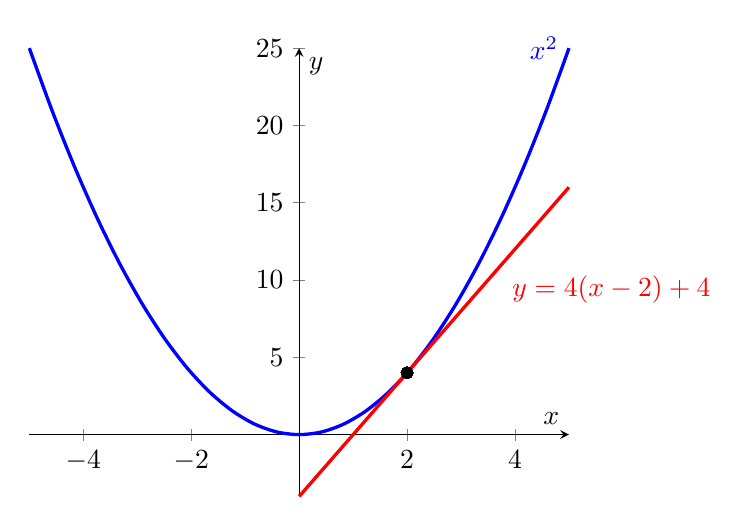
\begin{tikzpicture}[declare function = {
a = 2; % everything is calculated in terms of this
f(\x) = \x^2;
fp(\x) = 2*\x;
m = fp(a);}]
% OK, now I'm showing off, just to format label below
\pgfmathtruncatemacro{\m}{m}
\pgfmathtruncatemacro{\a}{a}
\pgfmathtruncatemacro{\fa}{f(a)}
% 
\begin{axis}[restrict y to domain = -5:25,
axis lines=middle,
xlabel={$x$},ylabel={$y$},clip=false]
\addplot[very thick,blue,smooth]{f(x)} node[left]{$x^2$};
\addplot[very thick,red]{fp(a)*(x-a)+f(a)} 
         node[pos=0.75,below right]{$y=\m(x-\a)+\fa$};
\addplot[only marks] ({a},{f(a)});
\end{axis}
\end{tikzpicture}%
~~
\tikzcount
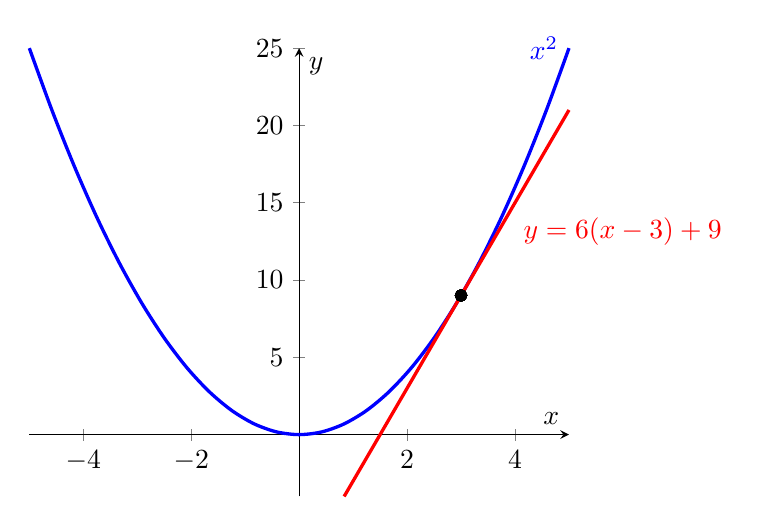
\begin{tikzpicture}[declare function = {
a = 3; % this is the ** only ** change from above
f(\x) = \x^2;
fp(\x) = 2*\x;
m = fp(a);}]
\pgfmathtruncatemacro{\m}{m}
\pgfmathtruncatemacro{\a}{a}
\pgfmathtruncatemacro{\fa}{f(a)}
% 
\begin{axis}[restrict y to domain = -5:25,
axis lines=middle,
xlabel={$x$},ylabel={$y$},clip=false]
\addplot[very thick,blue,smooth]{f(x)} node[left]{$x^2$};
\addplot[very thick,red]{fp(a)*(x-a)+f(a)} 
         node[pos=0.75,below right]{$y=\m(x-\a)+\fa$};
\addplot[only marks] ({a},{f(a)});
\end{axis}
\end{tikzpicture}
\end{center}
I did show off a little in that example to get the variables stored in
a format that I could use in the label.  Ordinarily those variables
and functions (i.e.\ "a", "f", "fp", "m") are only going to be usable
inside coordinates (and "domain"s, and maybe a few other places \dots\
but not in ``regular'' LaTeX places that are interpeted as something
to print).  But the PGF math engine can use them, and so I looked up
the command for storing them into macros which could then be used
elsewhere.  Beware: the internal PGF math engine is not really user
friendly, and this is one of the only times I've ever used it.
Ordinarily I would just type in the label for the tangent line as
"$y=4(x-2)+4$".

\subsubsection{A piecewise graph}
In 2023 a member of my department asked me for help in re-creating an
example from a book about a function defined by a graph (the problem
probably asked for an estimate of velocity at each marked point).  At
the time I didn't know "pgfplots" and so I created it in ``raw'' Tikz.
As a result a few things were harder: (1) I created a style for
marking points, (2) I had to scale the numbers in the graph to more
suitable numbers in Tikz, (3) I added labels to the axes myself, (4) I
repeated a math formula in two different parts.  Now that I know
"pgfplots" I can create the result more easily:
\begin{center}
\begin{minipage}{0.5\columnwidth}
\begin{latex}[xleftmargin=0in,basicstyle=\color{blue!75!black}\small\tt]
\tikzset{point/.style={fill=black,circle,
       inner sep =1.5pt}}
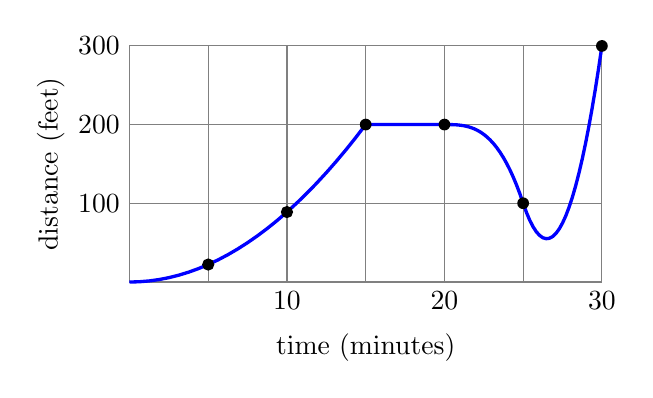
\begin{tikzpicture}
\draw[gray,thin] (0,0)  grid (6,3);
\draw[blue, very thick]
   plot[domain=0:3] (\x, {2/9*(\x^2)}) 
   node[point]{}                       
   -- (4,2)                            
   node[point]{}                       
   plot[domain=4:5]  (\x, {-1*((\x-4)^3)+2}) 
   node[point]{}                             
   plot[domain=5:6]  (\x,{5*(\x^2)-53*\x+141}) 
   node[point]{};                            
\draw plot[only marks,mark=*,samples at ={1,2}]
    (\x, {2/9*(\x^2)});
\foreach \x/\label in {2/10,4/20,6/30} 
    \draw (\x,0) node[below] {$\label$};
\foreach \y/\label in {1/100,2/200,3/300} 
    \draw (0,\y) node[left] {$\label$};
\node[rotate=90] at (-1,1.5) {distance (feet)};
\node[below=15pt] at (3,0) {time (minutes)};
\end{tikzpicture}
\end{latex}
\end{minipage}%
%
\begin{minipage}{0.5\columnwidth}
\begin{latex}[basicstyle=\color{blue!75!black}\small\tt]
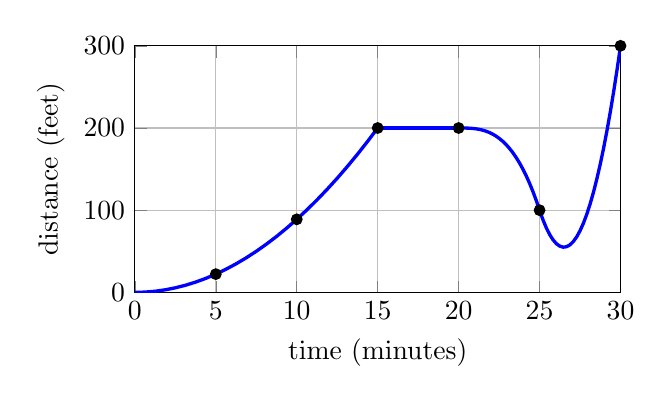
\begin{tikzpicture}
\begin{axis}[
  grid, x post scale=0.9, y post scale=0.55,
  every axis plot/.style={blue,very thick},
  xmin=0, xmax=30, ymin=0, ymax=300,
  declare function = {f(\x)=8/9*\x^2;},
  xlabel={time (minutes)},
  ylabel={distance (feet)}
  ]
\addplot [domain=0:15] {f(x)};
\addplot [domain=15:20] {200};
\addplot [domain=20:25] {-4/5*(x-20)^3+200};
\addplot [domain=25:30] {20*(x^2-53*x+705)};
\addplot [only marks, mark options={black, 
   mark size = 1.5pt}] coordinates {(5,{f(5)}) 
   (10,{f(10)}) (15,200) (20,200) (25,100) (30,300)}; 
\end{axis}
\end{tikzpicture}
\end{latex}
\end{minipage}
\end{center}

\begin{center}
\tikzcount
\tikzset{point/.style={fill=black,circle,inner sep =1.5pt}}
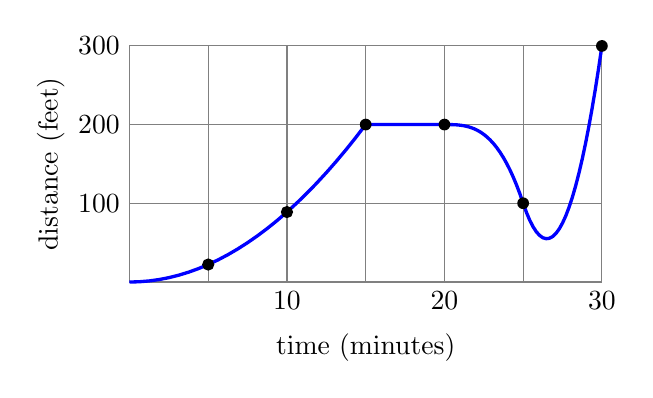
\begin{tikzpicture}
  \draw[gray,thin] (0,0)  grid (6,3);
  \draw[blue, very thick]
       plot[domain=0:3] (\x, {2/9*(\x^2)}) % first curve
       node[point]{}                       % point at x=3
       -- (4,2)                            % flat top
       node[point]{}                       % point at x=4
       plot[domain=4:5]  (\x, {-1*((\x-4)^3)+2}) % curve down to black point
       node[point]{}                             % point at x=5
       plot[domain=5:6]  (\x, {5*(\x^2) - 53*\x + 141}) % curve up to end
       node[point]{};                            % point at x=6
  \draw plot[only marks,mark=*,samples at ={1,2}](\x, {2/9*(\x^2)});
  \foreach \x/\label in {2/10,4/20,6/30} \draw (\x,0) node[below] {$\label$};
  \foreach \y/\label in {1/100,2/200,3/300} \draw (0,\y) node[left] {$\label$};
  \node[rotate=90] at (-1,1.5) {distance (feet)};
  \node[below=15pt] at (3,0) {time (minutes)};
\end{tikzpicture}
~~
\tikzcount
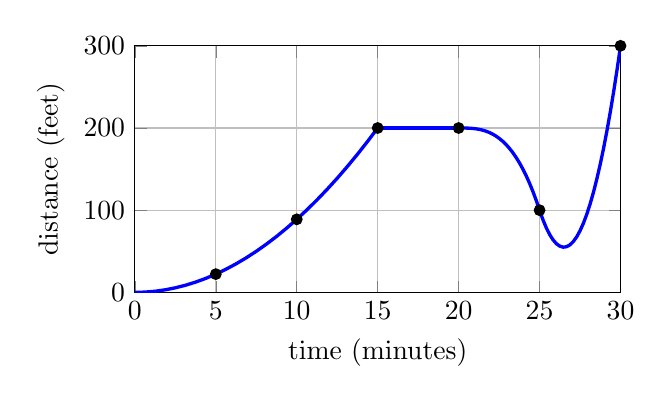
\begin{tikzpicture}
\begin{axis}[
  grid, x post scale=0.9, y post scale=0.55,
  every axis plot/.style={blue,very thick},
  xmin=0, xmax=30, ymin=0, ymax=300,
  declare function = {f(\x)=8/9*\x^2;},
  xlabel={time (minutes)},
  ylabel={distance (feet)}
  ]
\addplot [domain=0:15] {f(x)};
\addplot [domain=15:20] {200};
\addplot [domain=20:25] {-4/5*(x-20)^3+200};
\addplot [domain=25:30] {20*(x^2-53*x+705)};
\addplot [only marks, mark options={black,mark size = 1.5pt}] coordinates 
  {(5,{f(5)}) (10,{f(10)}) (15,200) (20,200) (25,100) (30,300)}; 
\end{axis}
\end{tikzpicture}
\end{center}
To reiterate, for me the improvement here is not so much that the code
is more compact (though it is), it's that it took less thought on my
part: it was easier.  It was easier to work with the coordinates I
could see, things like $(15,200)$ rather than scaling those in my head
to a smaller Tikz coordinate.  It was easier not to worry about adding
the tick labels.  It was easier to use the function "f(x)" (which I
could have done in Tikz, but didn't know about at the time).  


\subsubsection{Delta-Epsilon pictures}
Next, we illustrate how useful these function-programming features
are, by showing a picture that includes information for a
$\delta$-$\epsilon$ definition of the limit of a function .

\begin{latex}
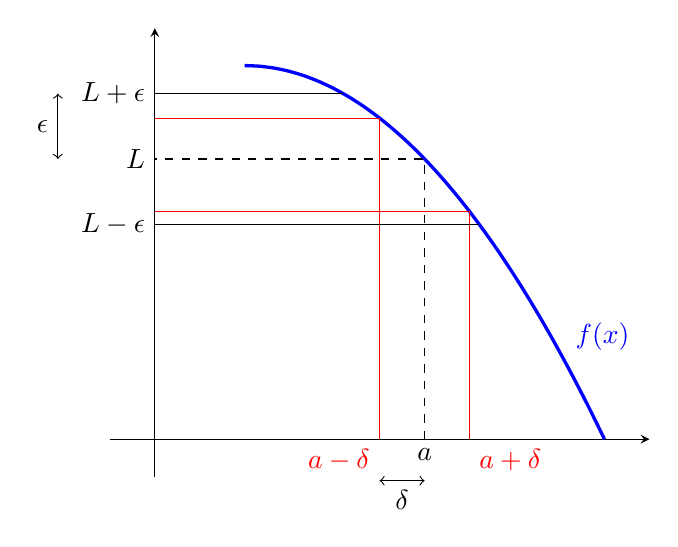
\begin{tikzpicture}[
  declare function = {
    a=3;
    f(\x) = -(\x-1)^2+16;
    L = f(a);
    eps = 2.8; % chosen to be visible
    del=0.5; % chosen to fit within eps
    x1 = sqrt(16-(L-eps))+1;
    x2 = sqrt(16-(L+eps))+1;
  }]
  \begin{axis}[
    axis lines = middle, xmin=0, enlargelimits,
    xtick=\empty,ytick=\empty, clip = false
    ]
    
% the actual function
\addplot[domain=1:5,smooth,very thick,blue]{f(x)} 
       node[pos=0.8,above right]{$f(x)$};

% the parts coming from the x-axis
\draw[dashed] (a,0) node[below]{$a$} -- (a,{f(a)}) -- 
           (0,{f(a)}) node[left]{$L$};
\draw[red] ({a-del},0) node[below left]{$a-\delta$}
       -- ({a-del},{f(a-del)}) -- (0,{f(a-del)});
\draw[red] ({a+del},0) node[below right]{$a+\delta$}
       -- ({a+del},{f(a+del)}) -- (0,{f(a+del)});

% the parts on the y-axis
\draw (0,{L-eps}) node[left]{$L-\epsilon$} -- (x1,{L-eps});
\draw (0,{L+eps}) node[left]{$L+\epsilon$} -- (x2,{L+eps});

% labeling the distance for delta and epsilon
\draw[<->] ({a-del},-15pt) -- node[below]{$\delta$} (a,-15pt);
\draw[<->] (-35pt,L) -- node[left]{$\epsilon$} (-35pt,{L+eps});
\end{axis}
\end{tikzpicture}
\end{latex}
%
\begin{center}
\tikzcount
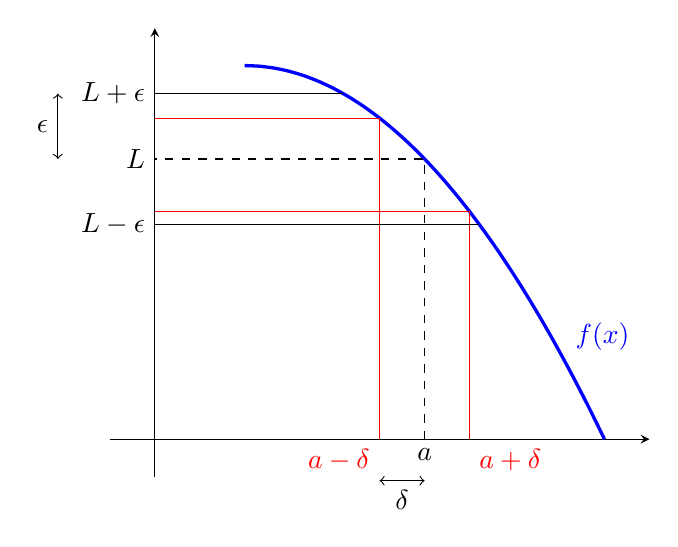
\begin{tikzpicture}[
  declare function = {
    a=3;
    f(\x) = -(\x-1)^2+16;
    L = f(a);
    eps = 2.8; % chosen to be visible
    del=0.5; % chosen to fit within eps
    x1 = sqrt(16-(L-eps))+1;
    x2 = sqrt(16-(L+eps))+1;
  }]
  \begin{axis}[
    axis lines = middle, xmin=0, enlargelimits,
    xtick=\empty,ytick=\empty, clip = false
    ]
    
% the actual function
\addplot[domain=1:5,smooth,very thick,blue]{f(x)} 
       node[pos=0.8,above right]{$f(x)$};

% the parts coming from the x-axis
\draw[dashed] (a,0) node[below]{$a$} -- (a,{f(a)}) -- 
           (0,{f(a)}) node[left]{$L$};
\draw[red] ({a-del},0) node[below left]{$a-\delta$}
       -- ({a-del},{f(a-del)}) -- (0,{f(a-del)});
\draw[red] ({a+del},0) node[below right]{$a+\delta$}
       -- ({a+del},{f(a+del)}) -- (0,{f(a+del)});

% the parts on the y-axis
\draw (0,{L-eps}) node[left]{$L-\epsilon$} -- (x1,{L-eps});
\draw (0,{L+eps}) node[left]{$L+\epsilon$} -- (x2,{L+eps});

% labeling the distance for delta and epsilon
\draw[<->] ({a-del},-15pt) -- node[below]{$\delta$} (a,-15pt);
\draw[<->] (-35pt,L) -- node[left]{$\epsilon$} (-35pt,{L+eps});
\end{axis}
\end{tikzpicture}
\end{center}
Notice a couple of things: (1) It was very convenient to have a
function that we could use to calculate $f(x)$.  (2) It was very
convenient to have a formula for the $x$-values corresponding to
$f\inv(L+\epsilon)$ and $f\inv(L-\epsilon)$ (we called them "x1" and
"x2" above).  (3) You can immediately get similar version of this
picture where we choose to make $\delta$ and $\epsilon$ smaller,
because the formulas for $f(x)$ and $f\inv(L\pm \epsilon)$ will
calculate the new values needed in the graph.  In the following graph,
all we changed compared to the previous code was to set "eps=1" and
"del=0.22"\,. (If we wanted to make $\epsilon$ smaller, we would
probably need to change a little more in the picture, such as the
labels for $L\pm \epsilon$, etc.)
\begin{center}
\tikzcount
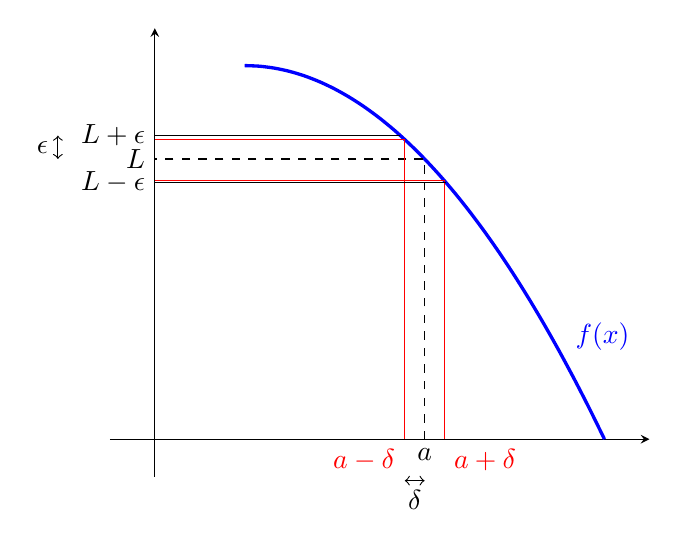
\begin{tikzpicture}[
  declare function = {
    a=3;
    f(\x) = -(\x-1)^2+16;
    L = f(a);
    eps = 1; % chosen to be visible
    del=0.22; % chosen to fit within eps
    x1 = sqrt(16-(L-eps))+1;
    x2 = sqrt(16-(L+eps))+1;
  }]
  \begin{axis}[
    axis lines = middle, xmin=0, enlargelimits,
    xtick=\empty,ytick=\empty, clip = false
    ]
    
% the actual function
\addplot[domain=1:5,smooth,very thick,blue]{f(x)} 
       node[pos=0.8,above right]{$f(x)$};

% the parts coming from the x-axis
\draw[dashed] (a,0) node[below]{$a$} -- (a,{f(a)}) -- 
           (0,{f(a)}) node[left]{$L$};
\draw[red] ({a-del},0) node[below left]{$a-\delta$}
       -- ({a-del},{f(a-del)}) -- (0,{f(a-del)});
\draw[red] ({a+del},0) node[below right]{$a+\delta$}
       -- ({a+del},{f(a+del)}) -- (0,{f(a+del)});

% the parts on the y-axis
\draw (0,{L-eps}) node[left]{$L-\epsilon$} -- (x1,{L-eps});
\draw (0,{L+eps}) node[left]{$L+\epsilon$} -- (x2,{L+eps});

% labeling the distance for delta and epsilon
\draw[<->] ({a-del},-15pt) -- node[below]{$\delta$} (a,-15pt);
\draw[<->] (-35pt,L) -- node[left]{$\epsilon$} (-35pt,{L+eps});
\end{axis}
\end{tikzpicture}
\end{center}






%%% Local Variables:
%%% mode: latex
%%% TeX-master: "../pgfplots_tutorial"
%%% End:
